% !TEX encoding = UTF-8 Unicode
\documentclass[a4j,11pt,report]{jsbook}
\usepackage[dvipdfmx]{graphicx}
\usepackage{tabularx}
\usepackage{fancybox}
\usepackage{ascmac}
\usepackage{amsmath,amssymb,amsthm}
\usepackage[dviout]{graphicx}
\usepackage{here}
\usepackage{bm}
\usepackage[dvipdfmx]{graphicx}
\usepackage{bmpsize}

\bibliographystyle{ipsjsort}
%\bibliographystyle{jplane}

\setlength{\topmargin}{-1in}
\addtolength{\topmargin}{5mm}
\setlength{\headheight}{5mm}
\setlength{\headsep}{0mm}
\setlength{\textheight}{\paperheight}
\addtolength{\textheight}{-25mm}
\setlength{\footskip}{5mm}

\newcommand{\frontpage}[3]{%
\title{卒業論文\\ \vspace{3em}\\{\huge #1}\\ \\#2\vspace{15em}}%
\author{{\huge 成蹊大学理工学部情報科学科}\\ \\{\huge #3}}%
\date{}
\maketitle
\clearpage
\thispagestyle{empty}

\clearpage
}



\newcommand{\point}[1]{
\begin{itembox}[l]{ポイント}
  #1
\end{itembox}
}

\begin{document}

\frontpage  % 以下の各項目を自分のテーマにあわせて修正する.
{計算問題の特徴分布に基づく類題選出による\\自己学習支援}
{Self Learning Support by Automatic Selection of Calculation Exercises based on Feature Distribution of Exercises}
{S152114 宮地 雄也}

\chapter*{要旨}
\thispagestyle{empty}
\if0
\point{
序論と結論の内容をもとに研究の内容をまとめる.
\begin{itemize}
  \item 問いは何か??
  \item 主張は何か??
  \item 結果はどうだったのか?
  \item 得られた成果の意義は?
\end{itemize}
}
\fi
\tableofcontents
\thispagestyle{empty}
\clearpage
\thispagestyle{plain}
\setcounter{page}{1}

\chapter{序論 \label{ch:introduction}}

\if0
\point{
問題提起を行う.
解く価値があり,簡単には解けず,誰も解いていない問題を扱っていることがわかるようにする.
\begin{itemize}
  \item どういう問題に取り組んだのか?
  \item その問題を解くことがなぜ重要なのか? 社会的意義(有用性)・学術的意義(問題の面白さ)
  \item その問題はどこが難しいのか? なぜこれまで解かれていなかったのか? これまではどうしていたのか?
  \item その問題をどのようなアプローチで解こうとしたのか? なぜそうしたのか?
\end{itemize}
}
\fi

昨今,小・中学生の理系離れが問題視されている.平成30年度全国学力・学習状況調査(全国学力テスト)の結果では平均正答率は小学校では算数Bが51.7\%,中学校数学では47.6\%とどちらも最も低く,ついで国語,理科の順で正答率が低い.
小中どちらとも理系教科の習熟度が低いことを示している.
この要因の一つに,数学は一つの計算方法が様々な分野に横断していくことが一度,苦手を生んでしまったらそこからの分野の理解度が下がり,次の分野での応用がきかないために連鎖的に苦手が蓄積することが原因ではないかと考えた.各単元のちょっとした積み残しが,後々,尾を引いていることが全国学力テストの結果から見て取れる.この状況を打破するには子供一人一人の苦手と向き合い,苦手と感じる前に理解していくしかない.
しかしながら,生徒と向き合うべき教師の労働時間は過酷を極めており,ベネッセ教育総合研究所の調査ではし小中高の教員の領導時間は増加の一途を辿っている.\cite{benesse_DateBook}
下の表は\cite{benesse_DateBook}での調査の結果の抜粋である.(\ref{tb:teacher_time})


\begin{center}
  \begin{table}[H]
    \begin{tabular}{|l|c|r|r|r|r|r|r|} \hline
      & 調査年 & 25歳以上 & 26〜30歳 & 31〜40歳 & 41〜50歳 & 51〜60歳  \\ \hline \hline
      & 2010 & 7:44 & 7:43 & 7:44 & 7:42 & 7:42 \\ \cline{2-7}
      出勤時間 & 2016 & 7:44 & 7:43 & 7:44 & 7:42 & 7:42 \\ \cline{2-7}\hline
      & 2010 & 19:30 & 19:40 & 19:10 & 18:57 & 18:31 \\ \cline{2-7}
      退勤時間 & 2016 & 20:00 & 19:54 & 19:26 & 19:05 & 18:46 \\ \cline{2-7}\hline
      & 2010 & 11時間46分 & 11時間57分 & 11時間26分 & 11時間15分 & 10時間49分  \\ \cline{2-7}
      学校にいる時間  & 2016 & 12時間26分 & 12時間18分 & 11時間46分 & 11時間26分 & 11時間06分 \\ \cline{2-7}\hline
    \end{tabular}

    \caption{出勤時刻・退勤時刻・学校にいる時間(平均時間、経年比較(教員年齢別〔公立全体〕))}
    \label{tb:teacher_time}
  \end{table}
\end{center}

表\ref{tb:teacher_time}によると,教員の労働時間は2010年に比べて2016年の方が各年次とも増加しており,教員のやることが増えている一方で
,主であるはずの教材研究や教務準備に時間が避けていないことを示している.
この状況では先生が生徒一人一人に時間をさき,指導することは難しい現状がつづいている.

この打開策として,IT技術駆使した個人別最適化学習に注目が集まっている,
しかし,教育の情報は,生徒の情報と結びついている個人情報なためオープン化できず,現在でているサービスでは各サービス利用者の利用状況からデータを取得し,その運用に利用しているため一部の王手企業が情報を独占している.
そこで個人の統計データではなく,解く数式の方に着目し,計算式自体の特徴を抽出し,間違えた問題と同様の特徴を持つ問題が復習する類題として最適なのではないかという仮定のもと,本論文では数式の特徴を掴むために自然言語処理の分野で使用される分散表現を適用し,さらに再起ニューラルネットワークを用いて数式ベクトルを作り出すことを目標とし,そのベクトルを用いて実際に復習問題生成を行った.

\chapter{分散表現\label{ch:Distributed representation}}
自然言語処理ではコンピューターで演算するために各単語を判別するために単語一つ一つをonehotベクトルというものに置き換える.
onehotベクトルとはある語彙数$V$の文章の中の単語$w_{i}$がある時,次元数$V$のベクトルに対し$i$番目の要素のみ1で残りが全て0になっているベクトルのことである.(\ref{onehot})

\begin{equation}
  \label{onehot}
  \bm{A} = \left(
  \begin{array}{c}
    0 \\
    0 \\
    1 \\
    \vdots \\
    0
  \end{array}
  \right)
  \quad \text{(i = 3 の時)}
\end{equation}


これにより単語一つ一つを別々のベクトルとして区別して表記することができる.
しかしonehotベクトルには問題点があり,一つ目として,ある単語の語彙数$V$が増加すると比例してonehotベクトルの次元$V$も大きくなり,処理に時間がかかる点がある.また二つ目としてonehotベクトルでは情報が0か1しかないので疎なベクトルができる.疎なベクトルとは次元数が大きくてもそのベクトルの持つ意味が薄いベクトルをさす,
このような問題を解決しようと考えられたのが分散表現である.

分散表現とは疎なonehotベクトルを密な密な実数値をの集合をベクトルそして扱い,その実数値で単語の意味を表そうとする手法である.
これにより疎なベクトルであった単語のベクトルを密な表現ができ,また,密度が上がることでベクトルの次元数を削減することができる.
以下.3手法はその分散表現を得るにあたって機械学習を応用した推論をベースとして編み出された手法である.

\clearpage
\section{Continuous Bag-of-Words Model\label{sec:CBOW}}
Continuous Bag-of-Words Model(以降,CBOWと略記)は\cite{SkipCBOW}で提唱された手法で,
ある単語数$\upsilon$の単語列$w_{0},w_{1},w_{2},\dots,w_{\upsilon-2},w_{\upsilon-1},w_{\upsilon}$がある時,単語$w_{t}$が文脈中で前後$m$単語をコンテキスト$C$とする時の前後$m$単語が共に共起する事前確率が増大するように学習するモデルである.(図\ref{fig:CBOWimage})


図\ref{fig:CBOWformula}より$w_{t}$をターゲットにした時の周辺単語$m$個を対象としたときの事後確率は式\ref{cobw同時確率}のように書くことができる.CBOWモデルでは式\ref{cobw同時確率}の最大化問題と見ることができる.
そこでCBOWの損失関数は,単に式\ref{cobw同時確率}の確率に対数を取りマイナスをつけ,最小化問題として解く.
式\ref{cbow_loss}はコーパス全体に拡張した形を示す.



\begin{figure}[H]
 \centering
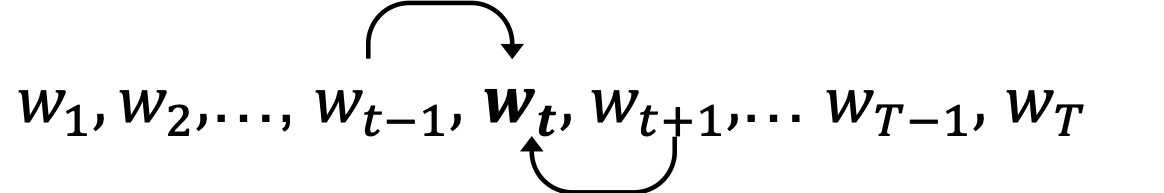
\includegraphics[width = 80mm]{image/cbow_w1w2wt-1wtwt+1.png}
 \caption{単語の列からターゲットとなる単語を推測する($m = 1$)}
 \label{fig:CBOWformula}
\end{figure}


\begin{equation}
  \label{cobw同時確率}
  \begin{array}{c}
    P(w_{t}|w_{t-m},...,w_{t+m})
  \end{array}
\end{equation}

\begin{equation}
  \label{cbow_loss}
  \begin{array}{c}
    L = -\frac{1}{T} \sum_{t = 0}^T \log P(w_{t}|w_{t-m},...,w_{t+m})
  \end{array}
\end{equation}

\begin{figure}[H]
 \centering
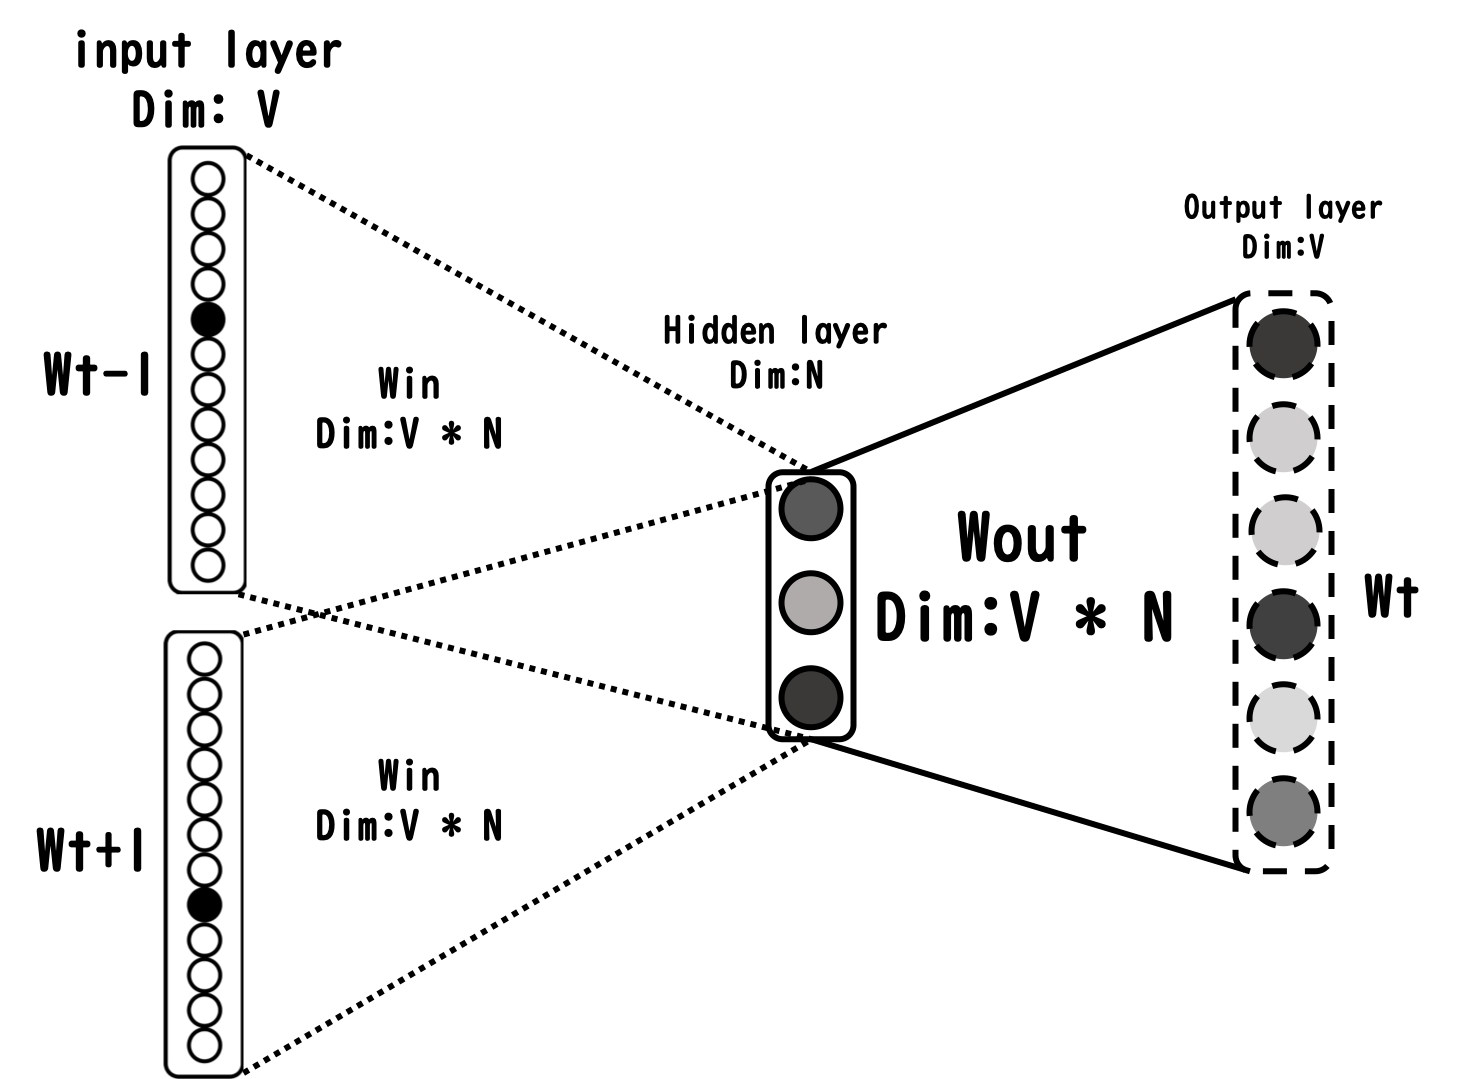
\includegraphics[width = 100mm]{image/CBOW_windowsize_1.png}
 \caption{CBOWのネットワーク構成モデル模式図($ m = 1$) }
 \label{fig:CBOWimage}
\end{figure}


\if0

\begin{figure}[H]
 \centering
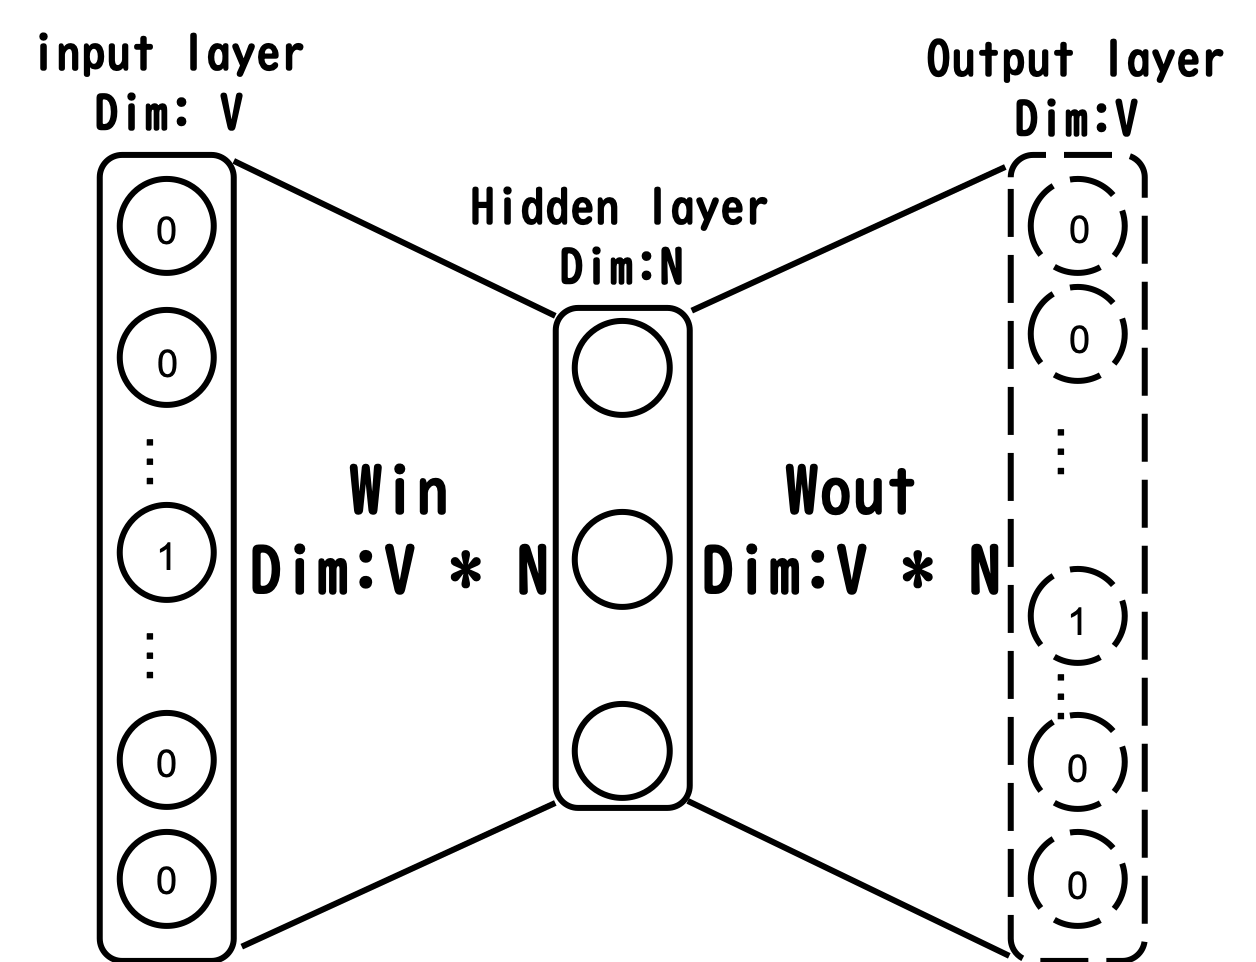
\includegraphics[scale = 0.5]{image/CBOW_image.png}
 \caption{次元圧縮のイメージ図 次元数$v$のベクトルに$V \times N $の埋め込み行列をかけて隠れ層のベクトルの次元を$N$次元に圧縮すことができる}
 \label{fig:CBOWimage}
\end{figure}
\fi

\clearpage

\section{Skip Gram \label{sec:SkipGram}}
Skip Gramは\cite{SkipCBOW}で紹介されている章\ref{sec:CBOW}で述べたCBOWとは別の手法である.
CBOWとは逆に中心の単語$w_{t}$から$m$個の周辺単語を推測するモデルである.
ネットワーク構成は図\ref{fig:SkipGramimage}のようになる.

\begin{figure}[H]
 \centering
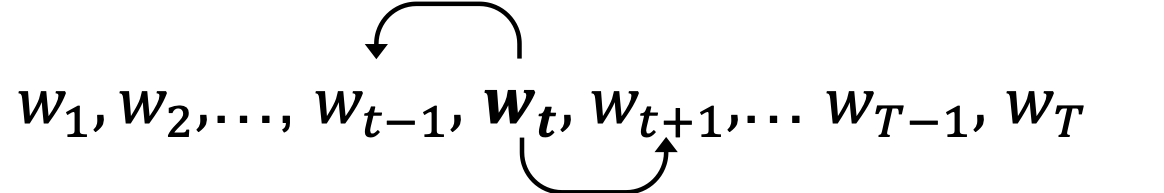
\includegraphics[width = 80mm]{image/skipgram_w1w2wt-1wtwt+1.png}
 \caption{単語の列からターゲットとなる単語を推測する($m = 1$)}
 \label{fig:Skipformula}
\end{figure}


\begin{figure}[H]
 \centering
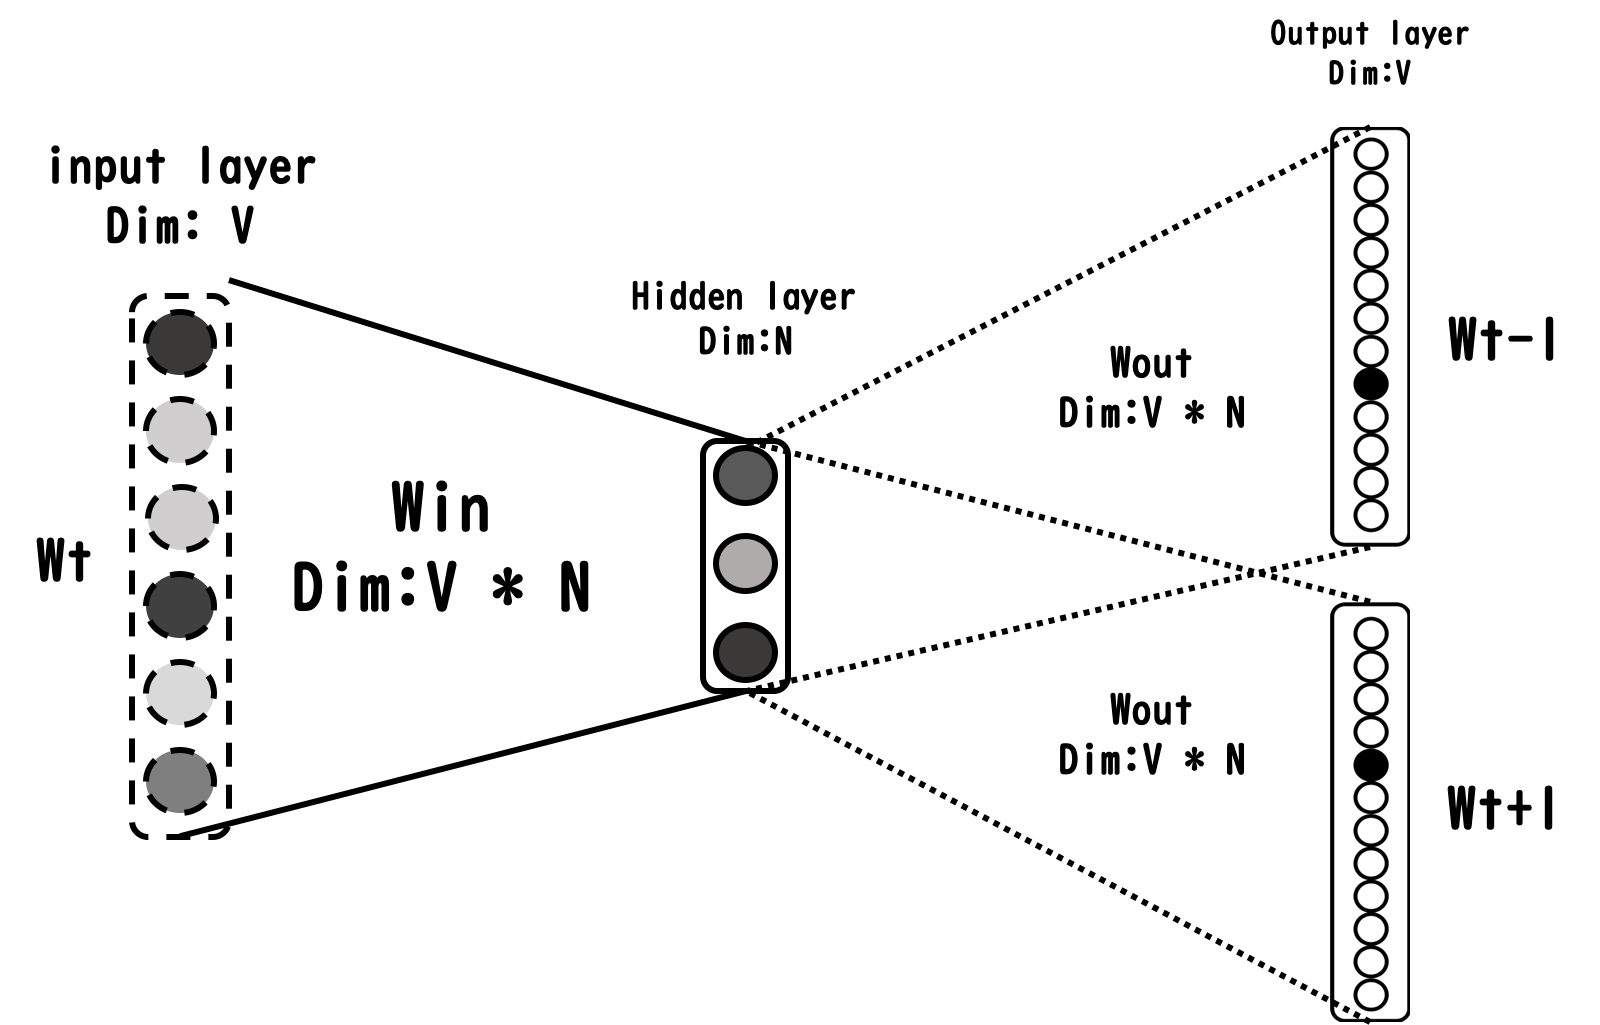
\includegraphics[width = 100mm]{image/SkipGram_windowsize_1.png}
 \caption{SkipGramのネットワーク構成モデル模式図($ m = 1$) }
 \label{fig:SkipGramimage}
\end{figure}



ある単語$w_{t}$が入力層に入力され,周辺単語の$w_{t-m},...,w_{t+m}$を推測する時,その全てが同時に起こる確率は式\ref{skip_probality}となる.

\begin{equation}
  \label{skip_probality}
  \begin{array}{c}
  P(w_{t-m},...,w_{t+m}|w_{t})
  \end{array}
\end{equation}

ここでSkipGramモデルは$w_{t-m},...,w_{t+m}$のそれぞれのあいだに関係性がないと仮定し,交差エントロピーを用いて損失関数(式\ref{skip_lossfunc})を定義する.

\begin{equation}
  \label{skip_lossfunc}
  \begin{split}
    \log P(w_{t-m},...,w_{t+m}|w_{t} ) &= -\log \prod_{k = 0}^m P(w_{t-k}|w_{t})   \\
                                       &= - \sum_{k = 0}^m \log P(w_{t-k} | w_{t})
  \end{split}
\end{equation}

そして式\ref{skip_lossfunc}をコンテキスト$C$をコーパス全体に拡張すると式\ref{skip_loss}となり,この式を学習によって最小化していく.

\begin{equation}
  \label{skip_loss}
  \begin{split}
    \sum_{C} \log P(w_{t-m},...,w_{t+m}|w_{t} ) &= \sum_{C} -\log \prod_{k = 0}^m P(w_{t-k}|w_{t})   \\
                                       &= - \sum_{C} \sum_{k = 0}^m \log P(w_{t-k} | w_{t})
  \end{split}
\end{equation}




\if0
\section{GloVe \label{sec:GloVe}}
\fi


\chapter{LSTM(Long short-term memory)\label{ch:LSTM}}
順伝播ニューラルネットワークでは前の情報はつかわないため文章や音声など,一つ前の情報に影響を受けるデータに対しては有用ではない.
そこで,ある時刻$t$の出力の際,過去の情報も扱う再起ニューラルネットワーク(以降 RNN と省略)というものが発案された.
これは時刻$t$の入力を$x_{t}$とする時,各ネットワークは過去の情報を記憶しているようにみなすことができる.
しかしながら通常のRNNの場合,時間が経つほどに魔の情報は薄れていく勾配消失が起こることがあった.
これを解決しようとしたのが記憶情報ごとにメモリーの役割を果たすネットワークを分けたLong short-term memory(以降,LSTMと省略)というモデルである.






\if0
\chapter{Attention\label{ch:Attention}}
これからね
\fi


\chapter{提案手法(章題は変える)\label{ch:method}}
\if0
\point{
自分の提案する解決方法を説明する.
\begin{itemize}
  \item 章題は適切なものに変えること.章をわけてもよい.
  \item 必ず具体例を用いること.
  \item 最初に問題を解く上で最も難しい点とそれを解決するアイデアを示す.
  \item 詳細については,全体の流れを示した後,各ステップについて説明する.
  \item 検討時に行った予備評価の結果があれば示す.
\end{itemize}
}
\fi

\section{システム全体の流れ}
<図をいれながら>



\section{計算式の特徴量抽出}
\subsection{概要}
<idea>
(内容充実させる)
数式を分布化する際,そのベクトルの中に数式の特徴を入れ込んだベクトルを生成する手法が確立していない.そこで本論文では数式の各文字,記号を単語のようにみなし,onehotベクトルを作成し,それを埋め込み層で特徴を踏まえた低次元ベクトルに変換したのち,系列変換モデルで読み込むことで低次元で数式の特徴を掴んだベクトルを生成できないかと考えた.


<手法>
この考えを実現するために数式は我々が目にする$2x+3=5$, $\frac{3x-1}{2}+4=\frac{2}{5}$ではなく,テキスト化かつその特徴を強く受けた形に変換する必要がある.
そこで本論文では数式をある一定のルールの中でテキスト化されている{\TeX}形式の数式を用いる.
上記の計算式なら\verb#2x+3=5#,\verb#\frac{3x-1}{2}+4=\frac{2}{5}#とし,このテキストデータを用いて文字単位の埋め込んだベクトルを作成する.

実験を行った手法は以下の三種法で行い,それぞれ分布をpythonを用いて確認した.
\begin{itemize}
  \item CBOW
  \item SkipGram
  \item ...
\end{itemize}

onehotベクトルの置き方は
\begin{itemize}
  \item $[0,1,2, ... ,9,+,-,=,x ...]$ のように各数字,各記号に割り当てる方法
  \item 出てきた数字,数式の塊をonehotを置く方法($[0,1,2, ... 3.6,0.11,...=.+,-]$)
  \item 3桁までの数字,数式に現れる記号
\end{itemize}


\subsection{文字分布の入手}
予備実験として文字の分布を入れる
CBOW,SkipGram,(できれば groveも)

できればベクトルの足し引きとかできればword2vecの論文にもそうので結果を確かめたい.




<おまけだからさらっと>
\section{判定機}
今回提案するシステムではといたプリントを読み込みその結果を判別して間違った計算問題を見つけ,その類題を選出する.
\subsection{概要}


『文章で説明』


→ あと誤差も(データ取り直しています)

\clearpage










\chapter{結果とその検討 \label{ch:result}}

\point{
自分の提案する方法が序論で提起した問題を解決できているかを評価・分析する.
\begin{itemize}
  \item 目的.何を確認するためのものか
  \item 方法.そのためにどういう実験を行ったか? 実験環境・用いたデータとその選定理由・手順を示し,評価の適切性を論証すること.
  \item 結果.その結果はどうだったか? 表やグラフを用いてまとめる.表はTeX,グラフはexcelでなくpythonを用いて作成すること.
  \item 分析.その結果から何が言えるか? 達成できた点・不足している点を理由と共に述べ,原因を考察する.
\end{itemize}
}

\section{実験}
\subparagraph{計算式の特徴量抽出}
\begin{itemize}
  \item 目的.数式のベクトル表現は可能なのかどうか
  \item 方法.埋め込み層,ネットワーク構成を変えながらEncoder-Decoderで復元を試みる
  そのEncoderの出力値を数式ベクトルとしてみなし,pca,T-sneで二次元ベクトルに圧縮し図示する
  \item 結果.これから
  \item 分析.これから
\end{itemize}

\subparagraph{計算式の特徴量からの類題選出}
\begin{itemize}
  \item 目的.求めた計算式のベクトルから特徴を捉えた数式を選出できるか
  \item 方法.特徴量ベクトルからk近法で選出,ある生徒の間違えた一問から類題を選出し,実際にその問題を間違えていたかを確認,また,逆にあっていた問題からも同様な手法で確認
  \item 結果.これから
  \item 分析.これから
\end{itemize}
\section{評価}
\section{分析}
\section{検討}





\chapter{関連研究\label{ch:relatedwork}}
\point{
この研究に関連する他の研究を紹介し,この研究との違いを明確にする.

https://code.google.com/archive/p/word2vec/

https://techblog.asahi-net.co.jp/entry/2018/10/05/180310


}


\chapter{結論と今後の課題 \label{ch:conclusion}}
\if0
\point{
序論で提起した問いとそれに対する答えをまとめる.
\begin{itemize}
  \item 提案手法のアイデアおよび評価結果を振り返る.
  \item この研究で得られた知見をまとめる.
  \item 今後の課題について述べる.
\end{itemize}
}
\fi


\if0
\chapter{形式上の注意}

\begin{itemize}
  \item 文字コードはUTF-8に統一する.
  \item 論文ファイル名は\texttt{chishiro-thesis.tex},文献ファイル名は\texttt{chishiro.bib}のように名前\texttt{-thesis.tex}とする.
  \item 句読点は全角のカンマ,ピリオドを用いる.
  \item 英数字はすべて半角を用いる.ギリシャ文字は{\TeX}の定義を用いる.$\alpha, \beta, ...$
  \item カンマの前にはスペースを入れず,カンマの後はスペースをひとつ入れる.
  \item 数式は{\TeX}の数式機能を用いる.例: $x^2$,\[f(x) = x^2 + 2x + 1.\].
  \item プログラムテキストはタイプライターフォントを用いる(例: \texttt{hello}).
  \item 文章構成(章・節・小節・箇条書き)は{\TeX}の機能を用いて指定する.自分で見出しなどを作らない.
  \item 題目には研究目的・方法・対象を特徴づける情報を入れる.
  \item 図のタイトルは図の下,表のタイトルは表の上に書く.
  \item 図表番号の参照は\verb#\label#および\verb#\ref#を用いる.自分で図表番号を指定しない.
  \item 表は{\TeX},グラフはすべてpythonで作成する.
  \item 図表番号のない図は用いない.
  \item 参照の?は必ず取り除く.
  \item 段落は意味の区切りでわける.意図しない字下げが入った場合\verb#\noindent#を用いて修正する.
  \item 参考文献は10以上あげる.
\end{itemize}
\fi


\chapter*{謝辞 \label{ch:acknowledgement}}
\thispagestyle{empty}
\if
\point{
本のあとがきに相当する部分.半ページ 以上書く.
卒業研究に協力者してくれた方々へのお礼を忘れずに述べる.
}
\fi
\cite{ZeroDeep}


\bibliography{miyaji}
\end{document}
